\chapter{Simulación Circuital y Ensayos Experimentales}
\label{sec:simulacion_mediciones}

El presente capítulo aborda la validación del amplificador de instrumentación
diseñado a través de dos etapas complementarias: en primer lugar, la simulación
circuital para corroborar el modelo analítico en condiciones nominales; en
segundo lugar, el ensayo en laboratorio sobre la placa física implementada, a
fin de contrastar y comprobar los resultados esperados
frente al comportamiento real.

% =========================================================================
% PARTE 1: SIMULACIÓN CIRCUITAL
% =========================================================================
\section{Simulación Circuital}
\label{subsec:simulacion_ltspice}

Para evaluar el diseño analítico se implementó el circuito
completo en el software de simulación LTspice, empleando los modelos
provistos por Texas Instruments para la familia TL081/TL084
(\texttt{TL081.301}).

\subsection{Respuesta Temporal en Modo Diferencial}
A fin de evaluar la ganancia diferencial en la zona central plana de la banda pasante, se inyecta entre los terminales $e_1$ y $e_2$ una señal senoidal pura de amplitud $v_d = \SI{10}{\milli\volt}$ ($v_{d,\text{pp}} = \SI{20}{\milli\volt\text{pp}}$) a una frecuencia de $\SI{25}{\hertz}$. 

En la Figura~\ref{fig:sim_modo_dif} se presentan el circuito esquemático configurado en LTspice y la respuesta temporal en régimen permanente obtenida en el nodo de salida $V_o$.

\begin{figure}[!ht]
  \centering
  \begin{subfigure}[b]{0.88\textwidth}
    \centering
    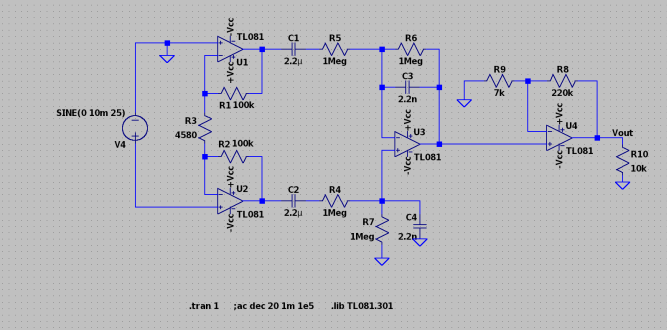
\includegraphics[width=\textwidth]{images/sim_crkt-modo_dif.png}
    \caption{Esquemático del circuito configurado en LTspice para excitación senoidal diferencial ($v_d = \SI{10}{\milli\volt}$, $f = \SI{25}{\hertz}$).}
    \label{subfig:sim_crkt_modo_dif}
  \end{subfigure}
  \vspace{0.4cm}
  \begin{subfigure}[b]{0.88\textwidth}
    \centering
    \resizebox{\linewidth}{!}{%
      \begin{tikzpicture}
  \pgfplotsset{
    scale only axis,
    xmin=0, xmax=120,
    xtick={0, 20, 40, 60, 80, 100, 120},
  }
  \begin{axis}[
    width=0.80\textwidth,
    height=5.2cm,
    grid=both,
    grid style={line width=.1pt, draw=gray!25},
    major grid style={line width=.2pt, draw=gray!45},
    xlabel={Tiempo [\unit{\milli\second}]},
    ylabel={Tensión diferencial de entrada $v_d$ [\unit{\milli\volt}]},
    ylabel style={color=red!80!black},
    yticklabel style={color=red!80!black},
    ymin=-30, ymax=40,
    ytick={-30, -20, -10, 0, 10, 20, 30, 40},
    axis y line*=left,
  ]
    \addplot[thick, dashed, color=red!80!black] table [x expr=\thisrow{time}*1000, y expr=\thisrow{vin}*1000] {sources/sim/sim_plot-ganancia_modo_dif.txt};
  \end{axis}
  \begin{axis}[
    width=0.80\textwidth,
    height=5.2cm,
    ylabel={Tensión de salida $V_o$ [\unit{\volt}]},
    ylabel style={color=blue!80!black},
    yticklabel style={color=blue!80!black},
    ymin=-18, ymax=24,
    ytick={-18, -12, -6, 0, 6, 12, 18, 24},
    axis y line*=right,
    axis x line=none,
    legend style={at={(0.98,0.95)}, anchor=north east, font=\footnotesize}
  ]
    \addlegendimage{thick, dashed, color=red!80!black}
    \addlegendentry{Entrada $v_d$ [\unit{\milli\volt}]}
    \addplot[thick, color=blue!85!black] table [x expr=\thisrow{time}*1000, y=vout] {sources/sim/sim_plot-ganancia_modo_dif.txt};
    \addlegendentry{Salida $V_o$ [\unit{\volt}]}
  \end{axis}
\end{tikzpicture}
%
    }
    \caption{Respuesta temporal en régimen permanente a $\SI{25}{\hertz}$.}
    \label{subfig:plot_sim_modo_dif}
  \end{subfigure}
  \caption{Simulación circuital y formas de onda del ensayo en modo diferencial a $\SI{25}{\hertz}$.}
  \label{fig:sim_modo_dif}
\end{figure}

Para la entrada diferencial aplicada de $\SI{10}{\milli\volt}$, la salida entrega una onda senoidal pura sin distorsión armónica con una amplitud de $v_{od} = \SI{13.36}{\volt}$ ($v_{od,\text{pp}} = \SI{26.73}{\volt\text{pp}}$), lo que determina una ganancia diferencial de:
\begin{equation*}
  A_{md,\text{sim}} = \frac{v_{od}}{v_d} = \frac{\SI{13.36}{\volt}}{\SI{10}{\milli\volt}} \approx 1336.3\ \text{V/V} \equiv \SI{62.52}{\decibel}
\end{equation*}

\subsection{Respuesta en Modo Común y Rechazo de Modo Común (RRMC)}
Para caracterizar la respuesta frente a interferencias de modo común (tales como la inducción capacitiva de la red de $\SI{50}{\hertz}$), se unen ambas entradas ($e_1 = e_2 = v_c$) y se aplica una señal senoidal de amplitud $v_c = \SI{1}{\volt}$ ($v_{c,\text{pp}} = \SI{2}{\volt\text{pp}}$) a $\SI{25}{\hertz}$.

En la Figura~\ref{fig:sim_modo_comun} se exhiben el esquemático de simulación correspondiente y la traza de tensión obtenida en la salida.

\begin{figure}[!ht]
  \centering
  \begin{subfigure}[b]{0.88\textwidth}
    \centering
    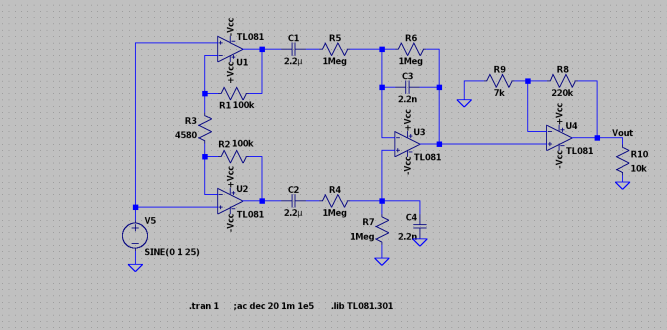
\includegraphics[width=\textwidth]{images/sim_crkt-modo_comun.png}
    \caption{Esquemático en LTspice configurado para modo común con entradas cortocircuitadas ($v_c = \SI{1}{\volt}$, $f = \SI{25}{\hertz}$).}
    \label{subfig:sim_crkt_modo_comun}
  \end{subfigure}
  \vspace{0.4cm}
  \begin{subfigure}[b]{0.88\textwidth}
    \centering
    \resizebox{\linewidth}{!}{%
      \begin{tikzpicture}
  \pgfplotsset{
    scale only axis,
    xmin=0, xmax=120,
    xtick={0, 20, 40, 60, 80, 100, 120},
  }
  \begin{axis}[
    width=0.80\textwidth,
    height=5.2cm,
    grid=both,
    grid style={line width=.1pt, draw=gray!25},
    major grid style={line width=.2pt, draw=gray!45},
    xlabel={Tiempo [\unit{\milli\second}]},
    ylabel={Tensión común de entrada $v_c$ [\unit{\volt}]},
    ylabel style={color=red!80!black},
    yticklabel style={color=red!80!black},
    ymin=-1.25, ymax=2.0,
    ytick={-1, -0.5, 0, 0.5, 1, 1.5},
    axis y line*=left,
  ]
    \addplot[thick, dashed, color=red!80!black] table [x expr=\thisrow{time}*1000, y=vin] {sim/sim_plot-ganancia_modo_com.txt};
  \end{axis}
  \begin{axis}[
    width=0.80\textwidth,
    height=5.2cm,
    ylabel={Tensión de salida residual $v_{oc}$ [\unit{\milli\volt}]},
    ylabel style={color=blue!80!black},
    yticklabel style={color=blue!80!black},
    ymin=-3.75, ymax=6.0,
    ytick={-3, -2, -1, 0, 1, 2, 3, 4, 5},
    axis y line*=right,
    axis x line=none,
    legend style={at={(0.98,0.95)}, anchor=north east, font=\footnotesize}
  ]
    \addlegendimage{thick, dashed, color=red!80!black}
    \addlegendentry{Entrada $v_c$ [\unit{\volt}]}
    \addplot[thick, color=blue!85!black] table [x expr=\thisrow{time}*1000, y expr=\thisrow{vout}*1000] {sim/sim_plot-ganancia_modo_com.txt};
    \addlegendentry{Salida $v_{oc}$ [\unit{\milli\volt}]}
  \end{axis}
\end{tikzpicture}
%
    }
    \caption{Respuesta temporal frente a interferencia de modo común a $\SI{25}{\hertz}$.}
    \label{subfig:plot_sim_modo_comun}
  \end{subfigure}
  \caption{Simulación circuital y atenuación de la señal de interferencia en modo común.}
  \label{fig:sim_modo_comun}
\end{figure}

Bajo esta condición, la amplitud observada a la salida es de apenas $v_{oc} \approx \SI{0.84}{\milli\volt}$ ($v_{oc,\text{pp}} = \SI{1.67}{\milli\volt\text{pp}}$), arrojando una ganancia en modo común de:
\begin{equation*}
  A_{mc,\text{sim}} = \frac{v_{oc}}{v_c} = \frac{\SI{0.84}{\milli\volt}}{\SI{1}{\volt}} \approx 8.36 \times 10^{-4}\ \text{V/V} \equiv -\SI{61.55}{\decibel}
\end{equation*}

A partir de ambas ganancias simuladas, la Relación de Rechazo de Modo Común
resulta:
\begin{equation*}
  \text{RRMC}_{\text{sim}} = 20 \log_{10} \left( \frac{A_{md,\text{sim}}}{A_{mc,\text{sim}}} \right) = 20 \log_{10} \left( \frac{1336.3}{8.36 \times 10^{-4}} \right) \approx \SI{124.07}{\decibel}
\end{equation*}

\FloatBarrier
\subsection{Respuesta en Frecuencia}
La respuesta en frecuencia completa del amplificador se obtuvo ejecutando la directiva \texttt{.ac dec 20 1m 1e5} en LTspice sobre un rango de $\SI{1}{\milli\hertz}$ a $\SI{100}{\kilo\hertz}$. En la Figura~\ref{fig:sim_bode_solo} se grafica la curva de módulo $|A_v(f)|$.

\begin{figure}[!ht]
  \centering
  \resizebox{0.90\textwidth}{!}{%
    \begin{tikzpicture}
  \begin{axis}[
    width=0.88\textwidth,
    height=6.2cm,
    xmode=log,
    xmin=1e-2, xmax=1e3,
    ymin=20, ymax=78,
    grid=both,
    grid style={line width=.1pt, draw=gray!25},
    major grid style={line width=.2pt, draw=gray!45},
    xlabel={Frecuencia [\unit{\hertz}]},
    ylabel={Ganancia $|A_v|$ [\unit{\decibel}]},
    legend style={at={(0.98,0.95)}, anchor=north east, font=\footnotesize}
  ]
    % Curva simulada
    \addplot[very thick, color=blue!85!black] table [x=freq, y=gain_db] {sources/sim/sim_plot-rta_frec.txt};
    \addlegendentry{Respuesta simulada $|A_v(f)|$}

    % Linea de referencia -3 dB (60.2 dB)
    \addplot[dashed, color=red!80!black, domain=1e-2:1e3] {60.21};
    \addlegendentry{Nivel a $-\SI{3}{\decibel}$ ($\SI{60.2}{\decibel}$)}

    % Lineas verticales en fL y fH
    \draw[dotted, thick, color=blue!80!black] (axis cs:0.0725, 20) -- (axis cs:0.0725, 60.21);
    \node[anchor=south west, font=\tiny, rotate=90, color=blue!80!black] at (axis cs:0.0725, 23) {$f_{L,\text{sim}} \approx \SI{0.07}{\hertz}$};

    \draw[dotted, thick, color=blue!80!black] (axis cs:72.32, 20) -- (axis cs:72.32, 60.21);
    \node[anchor=south west, font=\tiny, rotate=90, color=blue!80!black] at (axis cs:72.32, 23) {$f_{H,\text{sim}} \approx \SI{72.3}{\hertz}$};

    % Anotacion banda pasante
    \node[anchor=north, font=\scriptsize\bfseries, color=blue!90!black] at (axis cs:2.0, 50.0) {Banda pasante: $\approx \SI{63.2}{\decibel}$};
  \end{axis}
\end{tikzpicture}
%
  }
    \caption{Diagrama de Bode simulado: respuesta en frecuencia $|A_v(f)|$}
  \label{fig:sim_bode_solo}
\end{figure}

De la simulación se extraen los siguientes parámetros de respuesta frecuencial:
\begin{itemize}
  \item \textbf{Ganancia máxima en banda pasante:} $|A_v|_{\text{máx}} = \SI{63.21}{\decibel}$ ($1446.4\ \text{V/V}$)
  \item \textbf{Frecuencia de corte inferior:} $f_{L,\text{sim}} \approx \SI{0.072}{\hertz}$
  \item \textbf{Frecuencia de corte superior:} $f_{H,\text{sim}} \approx \SI{72.32}{\hertz}$
  \item \textbf{Ancho de banda:} $B_{\text{sim}} = f_H - f_L \approx \SI{72.25}{\hertz}$.
\end{itemize}

\FloatBarrier
\subsection{Fuente de señal electrocardiográfica} En esta simulación, el circuito fue excitado con una fuente de señal electrocardiográfica. Se implementó mediante una fuente por tramos continuos \texttt{PWL file=ecg\_source.txt} conectada a la entrada diferencial (Figura~\ref{fig:sim_ecg_completa}).

\begin{figure}[!ht]
  \centering
  \begin{subfigure}[b]{0.88\textwidth}
    \centering
    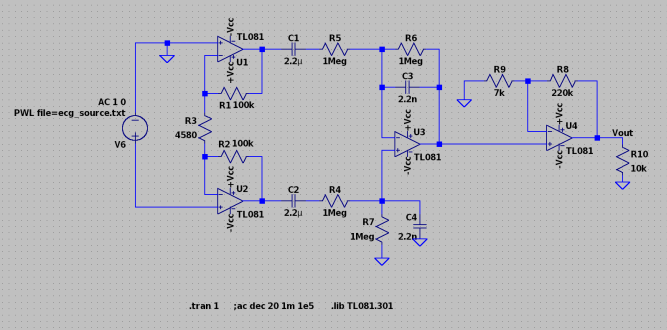
\includegraphics[width=\textwidth]{images/sim_crkt-fuente_ecg.png}
    \caption{Esquemático en LTspice con fuente \texttt{PWL file=ecg\_source.txt}.}
    \label{subfig:sim_crkt_ecg}
  \end{subfigure}
  \vspace{0.4cm}
  \begin{subfigure}[b]{0.88\textwidth}
    \centering
    \resizebox{\linewidth}{!}{%
      \begin{tikzpicture}
  \pgfplotsset{
    scale only axis,
    xmin=0, xmax=1.0,
  }
  \begin{axis}[
    width=0.80\textwidth,
    height=5.5cm,
    grid=both,
    grid style={line width=.1pt, draw=gray!25},
    major grid style={line width=.2pt, draw=gray!45},
    xlabel={Tiempo [\unit{\second}]},
    ylabel={Biopotencial de entrada $V_i$ [\unit{\milli\volt}]},
    ylabel style={color=red!80!black},
    yticklabel style={color=red!80!black},
    ymin=-2.0, ymax=8.4,
    ytick={-2, 0, 2, 4, 6, 8},
    axis y line*=left,
  ]
    \addplot[thick, dashed, color=red!80!black] table [x=time, y expr=\thisrow{vin}*1000] {sources/sim/sim_plot-fuente_ecg.txt};
  \end{axis}
  \begin{axis}[
    width=0.80\textwidth,
    height=5.5cm,
    ylabel={Tensión de salida $V_o$ [\unit{\volt}]},
    ylabel style={color=blue!80!black},
    yticklabel style={color=blue!80!black},
    ymin=-1.0, ymax=4.2,
    ytick={-1, 0, 1, 2, 3, 4},
    axis y line*=right,
    axis x line=none,
    legend style={at={(0.98,0.95)}, anchor=north east, font=\footnotesize}
  ]
    \addlegendimage{thick, dashed, color=red!80!black}
    \addlegendentry{Entrada $V_i$ [\unit{\milli\volt}]}
    \addplot[thick, color=blue!85!black] table [x=time, y=vout] {sources/sim/sim_plot-fuente_ecg.txt};
    \addlegendentry{Salida $V_o$ [\unit{\volt}]}
  \end{axis}
\end{tikzpicture}
%
    }
    \caption{Respuesta temporal al biopotencial cardíaco sintetizado.}
    \label{subfig:plot_sim_ecg}
  \end{subfigure}
  \caption{Simulación del circuito con señal electrocardiográfica.}
  \label{fig:sim_ecg_completa}
\end{figure}

Al inyectar una señal biopotencial diferencial de $V_{i,\text{pp}} \approx \SI{2.46}{\milli\volt\text{pp}}$ (con pico R de $\SI{2.04}{\milli\volt}$), la tensión de salida $V_o$ reproduce una forma de onda nítida de $V_{o,\text{pp}} \approx \SI{3.51}{\volt\text{pp}}$ (con pico R de $\SI{2.90}{\volt}$). Se comprueba:
\begin{enumerate}
  \item Preservación de la de la forma de onda QRS sin distorsión de flancos ni atenuación de altas frecuencias.
  \item Clara definición de las ondas lentas P y T.
  \item Eliminación absoluta de niveles de continua y centrado estable de la
      señal en $\SI{0}{\volt}$.
\end{enumerate}

% =========================================================================
% PARTE 2: ENSAYOS EXPERIMENTALES EN LABORATORIO
% =========================================================================
\clearpage
\section{Ensayos en laboratorio}
\label{subsec:ensayos_laboratorio}

Se procedió al diseño del amplificador en el programa KiCad (diseño de PCB
adjunto en anexo), a su montaje sobre una placa de circuito impreso
(Figura~\ref{fig:crkt_implementado}) y a su ensayo en laboratorio
(Figura~\ref{fig:medicion_lab}).

\begin{figure}[!ht]
  \centering
  \begin{subfigure}[b]{0.38\textwidth}
    \centering
    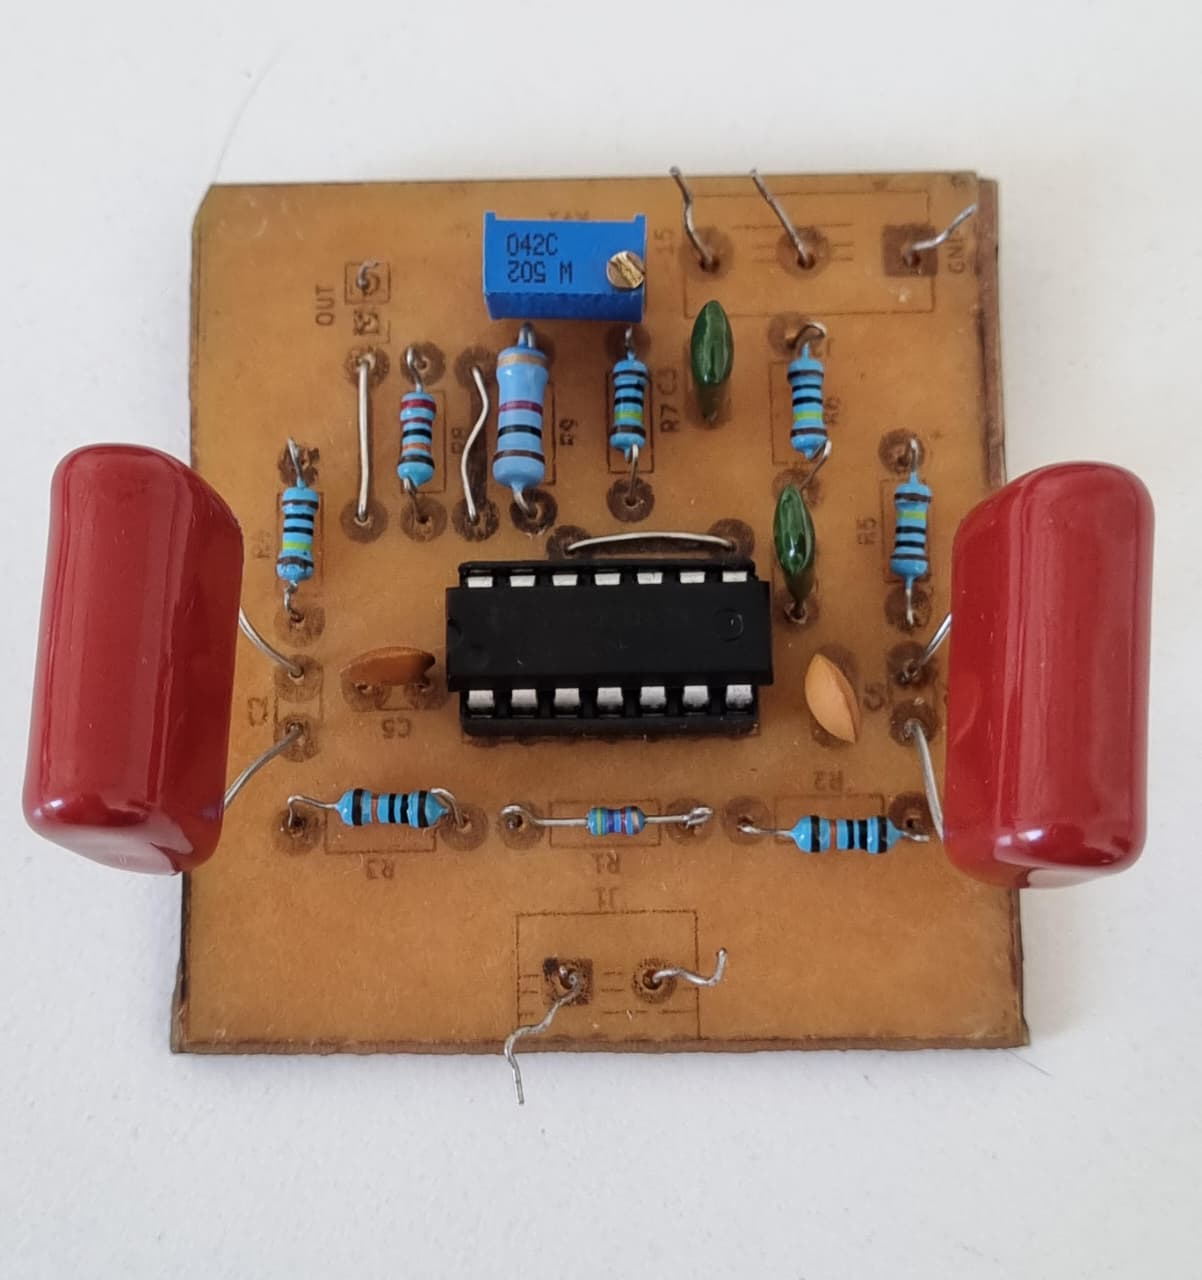
\includegraphics[height=4.6cm]{images/crkt_implementado.jpeg}
    \caption{Placa PCB ensamblada.}
    \label{fig:crkt_implementado}
  \end{subfigure}
  \hfill
  \begin{subfigure}[b]{0.58\textwidth}
    \centering
    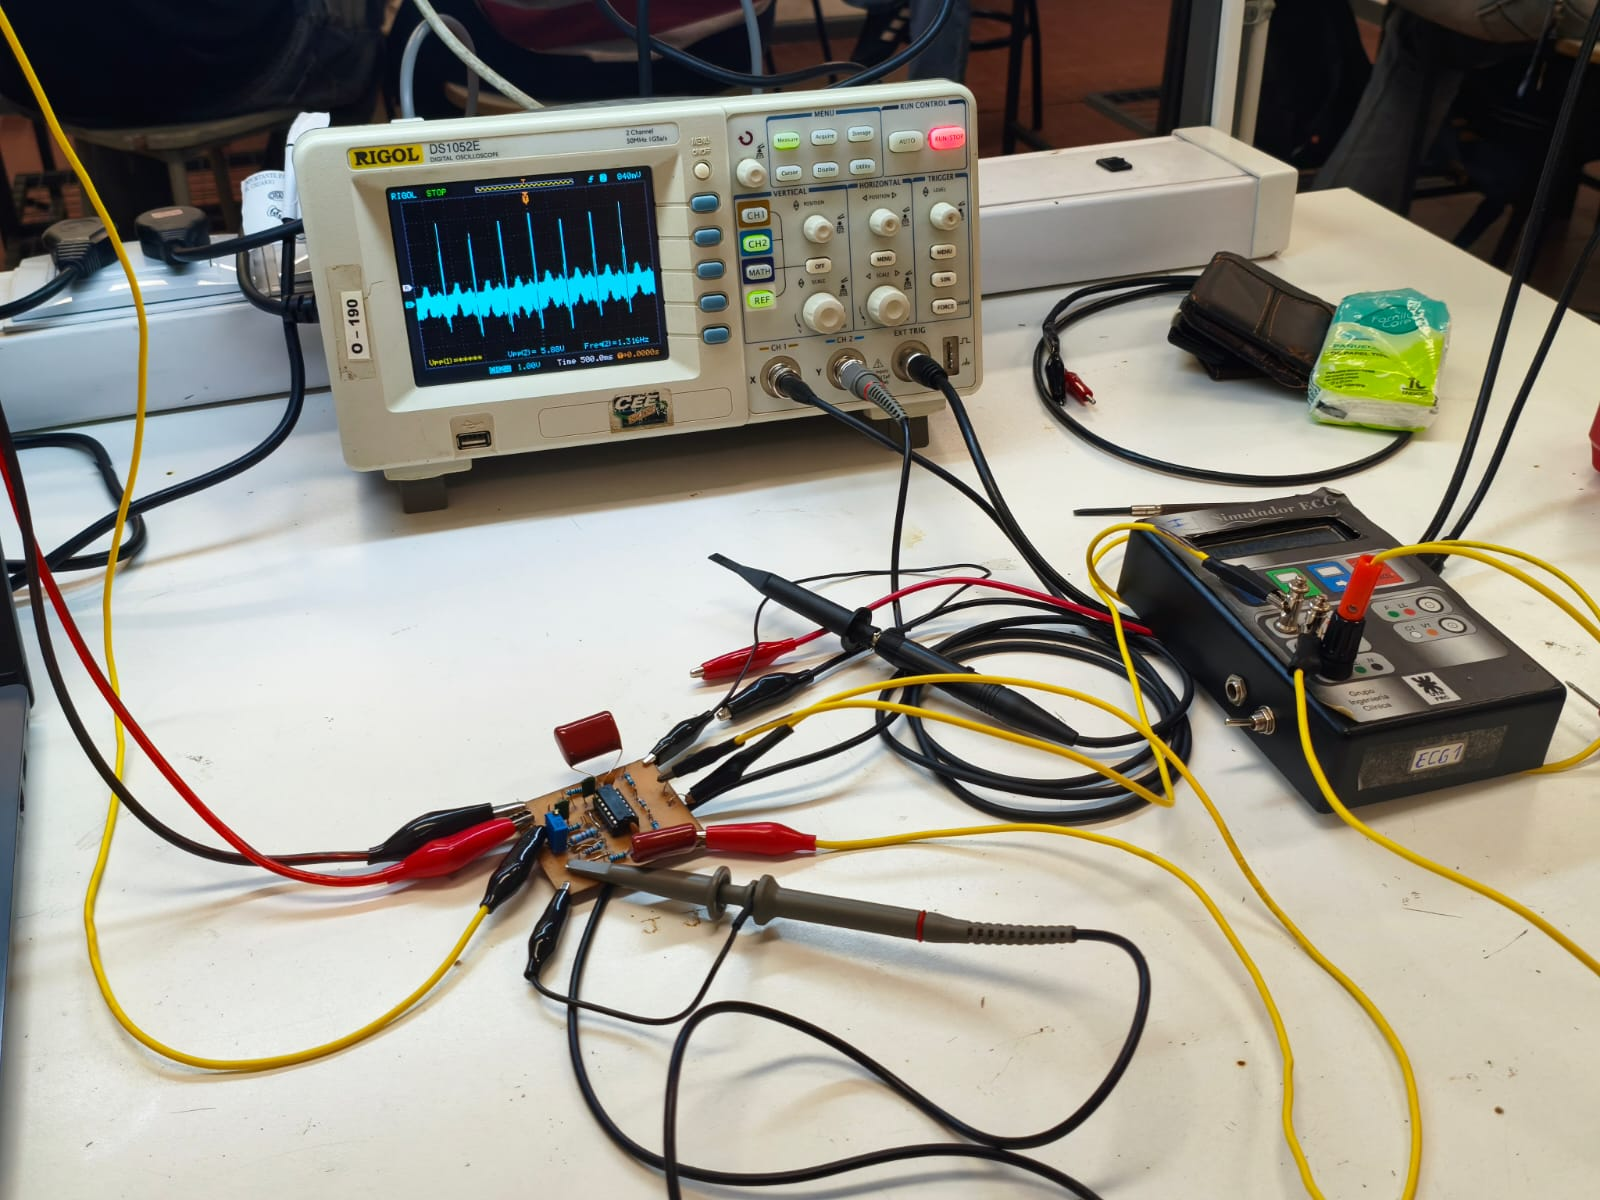
\includegraphics[height=4.6cm]{images/medicion_lab.jpeg}
    \caption{Ensayo experimental en banco de trabajo.}
    \label{fig:medicion_lab}
  \end{subfigure}
  \caption{Prototipo físico del amplificador de instrumentación: placa montada y puesta a prueba en banco de ensayo de laboratorio.}
  \label{fig:ensayo_prototipo}
\end{figure}

En las Figuras~\ref{crkt:medicion_rrmd}, \ref{crkt:medicion_rrmc} se detallan
las configuraciones instrumentales empleadas para los ensayos de modo
diferencial y modo común respectivamente.

\begin{figure}[!ht]
  \centering
  \begin{subfigure}[b]{0.48\textwidth}
    \centering
    \resizebox{\linewidth}{!}{%
      \begin{tikzpicture}[scale=0.95, transform shape]
  % Tarjeta exterior redondeada
  \draw[rounded corners=7pt, draw=gray!40, line width=0.8pt, fill=white] (-0.5, -0.3) rectangle (4.5, 2.7);

  % Triángulo Amplificador de Instrumentación (A.I.)
  \draw[line width=0.9pt] (1.9, 0.9) -- (1.9, 2.3) -- (2.8, 1.6) -- cycle;
  \node[font=\footnotesize\bfseries] at (2.2, 1.6) {A.I.};

  % Terminal superior (inversor) conectado a masa
  \draw[line width=0.7pt] (1.9, 2.1) -- (1.35, 2.1);
  \filldraw[black] (1.35, 2.1) circle (1.1pt);
  \draw[line width=0.7pt] (1.35, 2.1) -- (1.35, 1.6);

  % Terminal medio (referencia / masa)
  \draw[line width=0.7pt] (1.9, 1.6) -- (1.2, 1.6);
  % Masa de referencia del terminal medio
  \draw[line width=0.6pt] (1.2, 1.6) -- (1.2, 1.50);
  \draw[line width=0.8pt] (1.2-0.16, 1.50) -- (1.2+0.16, 1.50);
  \draw[line width=0.8pt] (1.2-0.10, 1.44) -- (1.2+0.10, 1.44);
  \draw[line width=0.8pt] (1.2-0.04, 1.38) -- (1.2+0.04, 1.38);

  % Terminal inferior (no inversor) conectado a generador
  \draw[line width=0.7pt] (1.9, 1.1) -- (0.65, 1.1) -- (0.65, 0.75);
  % Generador senoidal 10 mV, 25 Hz
  \draw[line width=0.7pt, fill=white] (0.65, 0.55) circle (0.18);
  \draw[line width=0.6pt] (0.65-0.11, 0.55) sin (0.65-0.055, 0.62) cos (0.65, 0.55) sin (0.65+0.055, 0.48) cos (0.65+0.11, 0.55);
  \node[anchor=west, align=left, font=\tiny] at (0.87, 0.55) {10 mV\\[-2pt]25Hz};
  % Masa del generador
  \draw[line width=0.7pt] (0.65, 0.37) -- (0.65, 0.30);
  \draw[line width=0.6pt] (0.65, 0.30) -- (0.65, 0.20);
  \draw[line width=0.8pt] (0.65-0.16, 0.20) -- (0.65+0.16, 0.20);
  \draw[line width=0.8pt] (0.65-0.10, 0.14) -- (0.65+0.10, 0.14);
  \draw[line width=0.8pt] (0.65-0.04, 0.08) -- (0.65+0.04, 0.08);

  % Salida Vo y Multímetro
  \draw[line width=0.7pt] (2.8, 1.6) -- (3.4, 1.6);
  \filldraw[black] (3.2, 1.6) circle (1.1pt);
  \node[above, font=\footnotesize] at (3.2, 1.63) {Vo};
  \draw[line width=0.7pt] (3.2, 1.6) -- (3.2, 1.18);

  % Símbolo de multímetro (voltímetro)
  \draw[line width=0.7pt, fill=white] (3.2, 0.95) circle (0.23);
  \node[font=\small\bfseries] at (3.2, 0.95) {V};
  \draw[-{Stealth[length=4pt, width=3pt]}, line width=0.5pt] (3.2-0.3, 0.95-0.3)
    -- (3.2+0.3, 0.95+0.3);

  % Masa del multímetro
  \draw[line width=0.7pt] (3.2, 0.72) -- (3.2, 0.60);
  \draw[line width=0.6pt] (3.2, 0.60) -- (3.2, 0.50);
  \draw[line width=0.8pt] (3.2-0.16, 0.50) -- (3.2+0.16, 0.50);
  \draw[line width=0.8pt] (3.2-0.10, 0.44) -- (3.2+0.10, 0.44);
  \draw[line width=0.8pt] (3.2-0.04, 0.38) -- (3.2+0.04, 0.38);
\end{tikzpicture}
%
    }
    \caption{Configuración para ganancia diferencial ($A_{md}$).}
    \label{crkt:medicion_rrmd}
  \end{subfigure}
  \hfill
  \begin{subfigure}[b]{0.48\textwidth}
    \centering
    \resizebox{\linewidth}{!}{%
      \begin{tikzpicture}[scale=0.95, transform shape]
  % Tarjeta exterior redondeada
  \draw[rounded corners=7pt, draw=gray!40, line width=0.8pt, fill=white] (-0.5, -0.3) rectangle (4.5, 2.7);

  % Triángulo Amplificador de Instrumentación (A.I.)
  \draw[line width=0.9pt] (1.9, 0.9) -- (1.9, 2.3) -- (2.8, 1.6) -- cycle;
  \node[font=\footnotesize\bfseries] at (2.2, 1.6) {A.I.};

  % Terminales de entrada unidos
  \draw[line width=0.7pt] (1.9, 2.1) -- (0.75, 2.1) -- (0.75, 1.1) -- (1.9, 1.1);
  \filldraw[black] (0.75, 1.4) circle (1.1pt);
  \draw[line width=0.7pt] (0.75, 1.4) -- (0.75, 0.75);

  % Terminal medio (referencia / masa)
  \draw[line width=0.7pt] (1.9, 1.6) -- (1.35, 1.6);
  % Masa de referencia del terminal medio
  \draw[line width=0.6pt] (1.35, 1.6) -- (1.35, 1.50);
  \draw[line width=0.8pt] (1.35-0.16, 1.50) -- (1.35+0.16, 1.50);
  \draw[line width=0.8pt] (1.35-0.10, 1.44) -- (1.35+0.10, 1.44);
  \draw[line width=0.8pt] (1.35-0.04, 1.38) -- (1.35+0.04, 1.38);

  % Generador senoidal en modo común
  \draw[line width=0.7pt, fill=white] (0.75, 0.55) circle (0.18);
  \draw[line width=0.6pt] (0.75-0.11, 0.55) sin (0.75-0.055, 0.62) cos (0.75, 0.55) sin (0.75+0.055, 0.48) cos (0.75+0.11, 0.55);
  \node[anchor=west, align=left, font=\tiny] at (0.97, 0.55) {1 Vpp\\[-2pt]25Hz};
  % Masa del generador
  \draw[line width=0.7pt] (0.75, 0.37) -- (0.75, 0.30);
  \draw[line width=0.6pt] (0.75, 0.30) -- (0.75, 0.20);
  \draw[line width=0.8pt] (0.75-0.16, 0.20) -- (0.75+0.16, 0.20);
  \draw[line width=0.8pt] (0.75-0.10, 0.14) -- (0.75+0.10, 0.14);
  \draw[line width=0.8pt] (0.75-0.04, 0.08) -- (0.75+0.04, 0.08);

  % Salida Vo y Multímetro
  \draw[line width=0.7pt] (2.8, 1.6) -- (3.4, 1.6);
  \filldraw[black] (3.2, 1.6) circle (1.1pt);
  \node[above, font=\footnotesize] at (3.2, 1.63) {Vo};
  \draw[line width=0.7pt] (3.2, 1.6) -- (3.2, 1.18);

  % Símbolo de multímetro (voltímetro)
  \draw[line width=0.7pt, fill=white] (3.2, 0.95) circle (0.23);
  \node[font=\small\bfseries] at (3.2, 0.95) {V};
  \draw[-{Stealth[length=4pt, width=3pt]}, line width=0.5pt] (3.2-0.3, 0.95-0.3)
    -- (3.2+0.3, 0.95+0.3);

  % Masa del multímetro
  \draw[line width=0.7pt] (3.2, 0.72) -- (3.2, 0.60);
  \draw[line width=0.6pt] (3.2, 0.60) -- (3.2, 0.50);
  \draw[line width=0.8pt] (3.2-0.16, 0.50) -- (3.2+0.16, 0.50);
  \draw[line width=0.8pt] (3.2-0.10, 0.44) -- (3.2+0.10, 0.44);
  \draw[line width=0.8pt] (3.2-0.04, 0.38) -- (3.2+0.04, 0.38);
\end{tikzpicture}
%
    }
    \caption{Configuración para ganancia en modo común ($A_{mc}$).}
    \label{crkt:medicion_rrmc}
  \end{subfigure}
  \caption{Esquemas instrumentales de conexión para la caracterización de rechazo de modo común en laboratorio.}
  \label{fig:setups_rrmc}
\end{figure}

\FloatBarrier
\subsection{Medición Experimental del RRMC}
La medición del Rechazo de Modo Común se efectuó inyectando señales a $\SI{25}{\hertz}$ (frecuencia central de la banda pasante, representativa de las perturbaciones de red de $\SI{50}{\hertz}$):
\begin{enumerate}
  \item \textbf{Modo Diferencial ($A_{md}$):} Con una entrada senoidal diferencial inyectada de $\SI{10}{\milli\volt}$, se midió una salida en el osciloscopio de $\SI{21.8}{\volt}$, resultando:
  \begin{equation*}
    A_{md,\text{med}} = \frac{\SI{21.8}{\volt}}{\SI{10}{\milli\volt}} = 2180.0\ \text{V/V} \equiv \SI{66.77}{\decibel}
  \end{equation*}
  \item \textbf{Modo Común ($A_{mc}$):} Con ambas entradas cortocircuitadas y excitadas con $\SI{1}{\volt}$, la tensión registrada a la salida fue de tan solo $\SI{25}{\milli\volt}$, arrojando:
  \begin{equation*}
    A_{mc,\text{med}} = \frac{\SI{25}{\milli\volt}}{\SI{1}{\volt}} = 0.0250\ \text{V/V} \equiv -\SI{32.04}{\decibel}
  \end{equation*}
  \item \textbf{RRMC experimental resultante:}
  \begin{equation*}
    \text{RRMC}_{\text{med}} = 20 \log_{10} \left( \frac{A_{md,\text{med}}}{A_{mc,\text{med}}} \right) = 20 \log_{10} \left( \frac{2180.0}{0.0250} \right) = 20 \log_{10}(87200) \approx \mathbf{\SI{98.80}{\decibel}}
  \end{equation*}
\end{enumerate}

En el Cuadro~\ref{tab:mediciones_rrmc} se encuentran los resultados
experimentales medidos frente a los valores obtenidos por simulación.

\begin{table}[!ht]
  \centering
  \caption{Comparativa de parámetros de modo diferencial, común y RRMC: valores simulados vs.\ mediciones experimentales en laboratorio.}
  \label{tab:mediciones_rrmc}
  \resizebox{\textwidth}{!}{%
  \begin{tabular}{|l|c|c|c|c|c|c|}
    \hline
    Parámetro de Ensayo & Frecuencia & $V_{\text{in}}$ aplicado & $V_{\text{out}}$ simulado & Ganancia Sim. & $V_{\text{out}}$ medido & Ganancia Medida \\ \hline
    Modo Diferencial ($A_{md}$) & $\SI{25}{\hertz}$ & $\SI{10}{\milli\volt}$ & $\SI{13.36}{\volt}$ & $1336.3\ \text{V/V}$ ($\SI{62.52}{\decibel}$) & $\SI{21.8}{\volt}$ & $2180.0\ \text{V/V}$ ($\SI{66.77}{\decibel}$) \\ \hline
    Modo Común ($A_{mc}$) & $\SI{25}{\hertz}$ & $\SI{1}{\volt}$ & $\SI{0.84}{\milli\volt}$ & $8.36 \times 10^{-4}$ ($-\SI{61.55}{\decibel}$) & $\SI{25}{\milli\volt}$ & $0.0250\ \text{V/V}$ ($-\SI{32.04}{\decibel}$) \\ \hline
    \multicolumn{3}{|l|}{\textbf{RRMC resultante (\unit{\decibel})}} & \multicolumn{2}{c|}{$\mathbf{\SI{124.07}{\decibel}}$ (Simulado)} & \multicolumn{2}{c|}{$\mathbf{\SI{98.80}{\decibel}}$ (Medido en laboratorio)} \\ \hline
  \end{tabular}%
  }
\end{table}

El valor medido de $\mathbf{\SI{98.80}{\decibel}}$ supera con amplio margen la
especificación mínima requerida ($\text{RRMC} \gg \SI{80}{\decibel}$). La
divergencia observada respecto al valor de simulación ($\SI{124.07}{\decibel}$)
se debe a que, mientras la simulación asume componentes ideales, en la placa
real las tolerancias y factores parásitos limita el RRMC práctico.

\subsection{Relevamiento Experimental de Respuesta en Frecuencia y Ancho de Banda}
Se ejecutó un barrido sinusoidal diferencial manteniendo la tensión de entrada constante en $V_{\text{in}} = \SI{10}{\milli\volt}$ en 21 frecuencias discretas distribuidas entre $\SI{0.1}{\hertz}$ y $\SI{2}{\kilo\hertz}$.

En el Cuadro~\ref{tab:barrido_frecuencia} se presenta el registro experimental completo obtenido en el laboratorio para el barrido en frecuencia, expresando la variación $\Delta$ en decibeles respecto a la frecuencia central de $\SI{25}{\hertz}$. El contraste con la respuesta teórica de simulación circuital se evalúa y visualiza en el diagrama de Bode comparativo de la Figura~\ref{fig:sim_bode_pgf}.

\begin{table}[!ht]
  \centering
  \renewcommand{\arraystretch}{1.12}
  \caption{Relevamiento experimental del barrido en frecuencia medido en laboratorio ($V_{\text{in}} = \SI{10}{\milli\volt}$).}
  \label{tab:barrido_frecuencia}
  \begin{tabular}{|c|c|c|c|c|}
    \hline
    $f$ (\unit{\hertz}) & $V_{\text{in}}$ (\unit{\milli\volt}) & $V_o$ medido (\unit{\volt}) & Ganancia (\unit{\decibel}) & $\Delta$ vs.\ $\SI{25}{\hertz}$ med. (\unit{\decibel}) \\ \hline
    0.1  & 10 & 19.00 & 65.58 & -1.19 \\ \hline
    0.25 & 10 & 22.80 & 67.16 & +0.39 \\ \hline
    0.5  & 10 & 23.60 & 67.46 & +0.69 \\ \hline
    1    & 10 & 23.60 & 67.46 & +0.69 \\ \hline
    2    & 10 & 23.60 & 67.46 & +0.69 \\ \hline
    5    & 10 & 23.60 & 67.46 & +0.69 \\ \hline
    10   & 10 & 23.40 & 67.38 & +0.62 \\ \hline
    20   & 10 & 22.80 & 67.16 & +0.39 \\ \hline
    25   & 10 & 21.80 & 66.77 & +0.00 \\ \hline
    50   & 10 & 19.60 & 65.85 & -0.92 \\ \hline
    75   & 10 & 16.40 & 64.30 & -2.47 \\ \hline
    100  & 10 & 13.50 & 62.61 & -4.16 \\ \hline
    125  & 10 & 11.60 & 61.29 & -5.48 \\ \hline
    150  & 10 & 10.00 & 60.00 & -6.77 \\ \hline
    200  & 10 & 8.00  & 58.06 & -8.71 \\ \hline
    300  & 10 & 5.30  & 54.49 & -12.28 \\ \hline
    500  & 10 & 3.32  & 50.42 & -16.35 \\ \hline
    700  & 10 & 2.32  & 47.31 & -19.46 \\ \hline
    1000 & 10 & 1.56  & 43.86 & -22.91 \\ \hline
    1500 & 10 & 1.10  & 40.83 & -25.94 \\ \hline
    2000 & 10 & 0.82  & 38.28 & -28.49 \\ \hline
  \end{tabular}
\end{table}

\clearpage

En la Figura~\ref{fig:sim_bode_pgf} se superponen los 21 puntos experimentales
medidos  sobre la curva de simulación, permitiendo verificar visualmente el
los resultados obtenidos.

\begin{figure}[!ht]
  \centering
  \begin{tikzpicture}
  \begin{axis}[
    width=0.96\textwidth,
    height=8.5cm,
    xmode=log,
    xmin=1e-2, xmax=3e3,
    ymin=20, ymax=85,
    ytick={20, 30, 40, 50, 60, 70, 80},
    grid=both,
    grid style={line width=.1pt, draw=gray!25},
    major grid style={line width=.2pt, draw=gray!45},
    xlabel={Frecuencia [\unit{\hertz}]},
    ylabel={Ganancia $|A_v|$ [\unit{\decibel}]},
    legend style={at={(0.98,0.96)}, anchor=north east, font=\footnotesize}
  ]
    % Curva simulada
    \addplot[very thick, color=blue!85!black] table [x=freq, y=gain_db] {sources/sim/sim_plot-rta_frec.txt};
    \addlegendentry{Respuesta simulada $|A_v(f)|$}

    % Puntos medidos en laboratorio
    \addplot[only marks, mark=*, mark size=2pt, color=red!80!black] coordinates {
      (0.1, 65.58)
      (0.25, 67.16)
      (0.5, 67.46)
      (1, 67.46)
      (2, 67.46)
      (5, 67.46)
      (10, 67.38)
      (20, 67.16)
      (25, 66.77)
      (50, 65.85)
      (75, 64.30)
      (100, 62.61)
      (125, 61.29)
      (150, 60.00)
      (200, 58.06)
      (300, 54.49)
      (500, 50.42)
      (700, 47.31)
      (1000, 43.86)
      (1500, 40.83)
      (2000, 38.28)
    };
    \addlegendentry{Medición en laboratorio}

    % Linea de referencia -3 dB simulada (60.2 dB)
    \addplot[dashed, thick, color=blue!70!gray, domain=1e-2:3e3] {60.21};
    \addlegendentry{Nivel sim. $-\SI{3}{\decibel}$ ($\SI{60.2}{\decibel}$)}

    % Lineas verticales en fL y fH simuladas
    \draw[dotted, thick, color=blue!80!black] (axis cs:0.0725, 20) -- (axis cs:0.0725, 60.21);
    \node[anchor=south west, font=\scriptsize, rotate=90, color=blue!80!black] at (axis cs:0.0725, 22) {$f_{L,\text{sim}} \approx \SI{0.07}{\hertz}$};

    % Linea vertical fH simulada (72.3 Hz)
    \draw[dotted, thick, color=blue!80!black] (axis cs:72.32, 20) -- (axis cs:72.32, 60.21);
    \node[anchor=south west, font=\scriptsize, rotate=90, color=blue!80!black] at (axis cs:72.32, 23) {$f_{H,\text{sim}} \approx \SI{72.3}{\hertz}$};

    % Linea vertical fH medida (82.2 Hz)
    \draw[dotted, thick, color=red!80!black] (axis cs:82.2, 20) -- (axis cs:82.2, 63.77);
    \node[anchor=north west, font=\scriptsize, rotate=90, color=red!80!black] at (axis cs:82.2, 23) {$f_{H,\text{med}} = \SI{82.2}{\hertz}$};
  \end{axis}
\end{tikzpicture}
%
  \caption{Bode $|A_v(f)|$: curva de simulación vs puntos medidos en laboratorio.}
  \label{fig:sim_bode_pgf}
\end{figure}

A partir del relevamiento experimental se comprueban los siguientes parámetros frente a los valores esperados:
\begin{itemize}
  \item \textbf{Ganancia en banda de paso:} La ganancia central a $\SI{25}{\hertz}$ fue de $\SI{66.77}{\decibel}$ ($2180.0\ \text{V/V}$), alcanzando una cota máxima plana de $\SI{67.46}{\decibel}$ ($2360.0\ \text{V/V}$) entre $\SI{0.5}{\hertz}$ y $\SI{5}{\hertz}$. Ambas superan holgadamente la cota mínima de diseño impuesta de $\ge \SI{60}{\decibel}$ ($1000\ \text{V/V}$).
  \item \textbf{Frecuencia de corte inferior ($f_L$):} Se corroboró que a $\SI{0.1}{\hertz}$ la respuesta ya se encuentra plenamente dentro de la banda útil ($\SI{65.58}{\decibel}$, con solo $-\SI{1.19}{\decibel}$ de atenuación respecto a $\SI{25}{\hertz}$), validando el bloqueo de continua y concordando con el polo teórico esperado de $f_L \approx \SI{0.07}{\hertz}$.
  \item \textbf{Frecuencia de corte superior ($f_H$):} La atenuación a $-\SI{3}{\decibel}$ respecto a la ganancia central ($\SI{66.77}{\decibel} - \SI{3.00}{\decibel} = \SI{63.77}{\decibel}$) se determinó experimentalmente en:
  \begin{equation*}
    f_{H,\text{med}} = \mathbf{\SI{82.2}{\hertz}}
  \end{equation*}
  La discrepancia del $+13.7\%$ frente al valor nominal esperado ($\SI{72.3}{\hertz}$) resulta totalmente justificada por la tolerancia comercial de los capacitores de poliéster ($C_4 = \SI{2.2}{\nano\farad} \pm 10\%$) y la dispersión resistiva.
  \item \textbf{Ancho de banda efectivo:} El ancho de banda medido resulta $\text{BW}_{\text{med}} = \mathbf{\SI{82.2}{\hertz}}$, cumpliendo con creces la banda requerida para el registro electrocardiográfico ($\SI{0.05}{\hertz}$ a $\SI{100}{\hertz}$).
\end{itemize}

\clearpage
\subsection{Síntesis y Comprobación frente a las Especificaciones de Diseño}
En el Cuadro~\ref{tab:sintesis_especificaciones} se resume la contrastación final entre los requerimientos de partida, los resultados calculados analíticamente, las simulaciones circuitales y las mediciones experimentales en laboratorio.

\begin{table}[!ht]
  \centering
  \caption{Síntesis comparativa final: especificaciones impuestas vs.\ cálculos analíticos, simulación en LTspice y mediciones de laboratorio.}
  \label{tab:sintesis_especificaciones}
  \resizebox{0.95\textwidth}{!}{%
  \begin{tabular}{|l|c|c|c|c|c|}
    \hline
    Parámetro de Diseño & Especificación & Cálculo Teórico & Simulación LTspice & Medición Laboratorio & Estado \\ \hline
    Ganancia diferencial ($A_{md}$) & $\ge \SI{60}{\decibel}$ ($1000\times$) & $\SI{63.00}{\decibel}$ ($1413\times$) & $\SI{62.52}{\decibel}$ ($1336\times$) & $\SI{66.77}{\decibel}$ ($2180\times$) & \textbf{Cumple} \\ \hline
    Frecuencia de corte inferior ($f_L$) & $0.05\text{ a } \SI{0.07}{\hertz}$ & $\SI{0.072}{\hertz}$ & $\SI{0.072}{\hertz}$ & Activo en $\SI{0.1}{\hertz}$ & \textbf{Cumple} \\ \hline
    Frecuencia de corte superior ($f_H$) & $70\text{ a } \SI{100}{\hertz}$ & $\SI{72.34}{\hertz}$ & $\SI{72.32}{\hertz}$ & $\SI{82.20}{\hertz}$ & \textbf{Cumple} \\ \hline
    Ancho de banda pasante ($\text{BW}$) & $70\text{ a } \SI{100}{\hertz}$ & $\SI{72.27}{\hertz}$ & $\SI{72.25}{\hertz}$ & $\SI{82.20}{\hertz}$ & \textbf{Cumple} \\ \hline
    Rechazo de Modo Común (RRMC) & $\gg \SI{80}{\decibel}$ & $\infty$ (ideal) & $\SI{124.07}{\decibel}$ & $\mathbf{\SI{98.80}{\decibel}}$ & \textbf{Cumple} \\ \hline
    Rechazo de continua ($A_v(0)$) & $\SI{0}{\decibel}$ (bloqueo) & $0\ \text{V/V}$ ($-\infty\ \text{dB}$) & $0\ \text{V/V}$ ($-\infty\ \text{dB}$) & Verificado ($V_{\text{offset}} \approx 0$) & \textbf{Cumple} \\ \hline
  \end{tabular}%
  }
\end{table}

Como balance general del proceso de validación, se comprueba que el prototipo
físico no solo satisface la totalidad de las pautas de diseño estipuladas, sino
que exhibe un desempeño altamente robusto frente a perturbaciones externas. La
concordancia cualitativa y cuantitativa entre el análisis analítico, el
comportamiento simulado en LTspice y las curvas relevadas en el banco
experimental demuestra la validez del diseño.
